%%%%%%%%%%%%%%%%%%%%%%%%%%%%%%%%%%%%%%%%%%%%%%%%%%%%%%%%%%%%%%%%%%%%%%%%
% Beamer Presentation - LaTeX - Template Version 1.0 (10/11/12)
% This template has been downloaded from: http://www.LaTeXTemplates.com
% License: % CC BY-NC-SA 3.0 (http://creativecommons.org/)
% Modified by Rahmat M. Samik-Ibrahim

% REV024: Wed 31 Jan 2024 10:00
% REV021: Mon 06 Feb 2023 00:00
% REV019: Thu 02 Feb 2023 00:00
% REV003: Mon 14 Feb 2022 21:00
% REV001: Mon 07 Feb 2022 18:00
% STARTX: Wed 14 Sep 2016 10:00
%%%%%%%%%%%%%%%%%%%%%%%%%%%%%%%

% PACKAGES AND THEMES 
\documentclass[aspectratio=169, xcolor=table, notheorems, hyperref={pdfpagelabels=false}]{beamer}
%%%%%%%%%%%%%%%%%%%%%%%%%%%%%%%%%%%%%%%%%%%%%%%%%%%%%%%%%%%%%%%%%%%%%%%%
% Beamer Presentation - LaTeX - Template Version 1.0 (10/11/12)
% This template has been downloaded from: http://www.LaTeXTemplates.com
% License: % CC BY-NC-SA 3.0 (http://creativecommons.org/)
% Modified by Rahmat M. Samik-Ibrahim
% REV419: Wed 24 Jul 2024 17:00
% REV383: Tue 12 Jul 2022 10:00
% REV316: Wed 14 Jul 2021 13:00
% REV198: Wed 13 Mar 2019 16:00
% REV005: Mon  2 Oct 2017 14:00
% STARTX: Thu 25 Aug 2016 14:00
%%%%%%%%%%%%%%%%%%%%%%%%%%%%%%%%%%%%%%%%%%%%%%%%%%%%%%%%%%%%%%%%%%%%%%%%%

%% ZCZC NNNN
\newtheorem{example}{Example}

%%%%%%%%%%%%%%%%%%%%%%%%%%%%%%%%%%%%%%%%%%%%%%%%%%%%%%%%%%%%%%%%%%%%%%%%%

\let\Tiny=\tiny
\mode<presentation> {
% The Beamer class comes with a number of default slide themes
% which change the colors and layouts of slides. Below this is a list
% of all the themes, uncomment each in turn to see what they look like.
%\usetheme{Boadilla}
\usetheme{Madrid}
% ZCZC %%%%%%%%%%%%%%%%%%%%%%%%%%%%%%%%%%%%%%%%%%%%%%%%%%%%%%%%%%%%%%%%%%
% \usetheme{default} \usetheme{AnnArbor} \usetheme{Antibes} \usetheme{Bergen}
% \usetheme{Berkeley} \usetheme{Berlin} \usetheme{CambridgeUS} 
% \usetheme{Copenhagen} \usetheme{Darmstadt} \usetheme{Dresden}
% \usetheme{Frankfurt} \usetheme{Goettingen} \usetheme{Hannover}
% \usetheme{Ilmenau} \usetheme{JuanLesPins} \usetheme{Luebeck}
% \usetheme{Malmoe} \usetheme{Marburg} \usetheme{Montpellier}
% \usetheme{PaloAlto} \usetheme{Pittsburgh} \usetheme{Rochester}
% \usetheme{Singapore} \usetheme{Szeged} \usetheme{Warsaw}
% NNNN %%%%%%%%%%%%%%%%%%%%%%%%%%%%%%%%%%%%%%%%%%%%%%%%%%%%%%%%%%%%%%%%%%
% As well as themes, the Beamer class has a number of color themes
% for any slide theme. Uncomment each of these in turn to see how it
% changes the colors of your current slide theme.
%\usecolortheme{orchid}
%\usecolortheme{rose}
%\usecolortheme{seagull}
%\usecolortheme{seahorse}
\usecolortheme{whale}
% ZCZC %%%%%%%%%%%%%%%%%%%%%%%%%%%%%%%%%%%%%%%%%%%%%%%%%%%%%%%%%%%%%%%%%%
%\usecolortheme{albatross} \usecolortheme{beaver} \usecolortheme{beetle}
%\usecolortheme{crane} \usecolortheme{dolphin} \usecolortheme{dove}
%\usecolortheme{fly} \usecolortheme{lily} \usecolortheme{wolverine}
% NNNN %%%%%%%%%%%%%%%%%%%%%%%%%%%%%%%%%%%%%%%%%%%%%%%%%%%%%%%%%%%%%%%%%%
% To remove the footer line in all slides uncomment this line
%\setbeamertemplate{footline} 
% To replace the footer line in all slides uncomment this line
%\setbeamertemplate{footline}[page number] 
% To remove the navigation symbols from the bottom uncomment this line
\setbeamertemplate{navigation symbols}{} 
}

\usepackage{array}       % ZCZC
\usepackage{amssymb}     % ZCZC
\usepackage{bold-extra}  % ZCZC
\usepackage{booktabs}    % Allows \toprule, \midrule and \bottomrule in tables
\usepackage{caption}
\usepackage[T1]{fontenc} % ZCZC << >>
\usepackage{graphicx}    % Allows including images
\usepackage{listings}    % listing
\usepackage{lmodern}     % ZCZC
\usepackage{perpage}     % reset footnote per page
\usepackage{geometry}    % ZCZC
\usepackage{adjustbox}   % ZCZC
\usepackage{multicol}    % ZCZC
\usepackage{multirow}    % ZCZC
\usepackage{pgf-pie}     % ZCZC pie chart

% \definecolor{links}{HTML}{2A1B81}
\definecolor{links}{HTML}{0011FF}
\hypersetup{colorlinks,linkcolor=,urlcolor=links}

% \usepackage{xcolor}
% \usepackage[colorlinks = true,
%             linkcolor = blue,
%             urlcolor  = blue,
%             citecolor = blue,
%             anchorcolor = blue]{hyperref}

\captionsetup[table]{name=Tabel}
\makeatletter
\def\input@path{{src/}}
\makeatother
\graphicspath{{src/}}      % src directory
\MakePerPage{footnote}     % reset page

% NNNN %%%%%%%%%%%%%%%%%%%%%%%%%%%%%%%%%%%%%%%%%%%%%%%%%%%%%%%%%%%%%%%%%%

%% % XXXXXXXXXXXXXXXXXXXXXXXXXXXXXXXXXXXXXXXXXXXXXXXXXXXXXXXXXXXXXXXXXXXXXXXXXX
%% % The short title appears at the bottom of every slide, 
%% % the full title is only on the title page
%% \title[Judul Pendek]{Judul Panjang dan Lengkap} 
%% \author{Cecak bin Kadal}
%% \institute[UILA]
%% {
%% University of Indonesia at Lenteng Agung \\ 
%% \medskip
%% \textit{cecak@binKadal.com}
%% }
%% \date{REV00 24-Aug-2016}
%% % \date{\today}
%% 

%% % XXXXXXXXXXXXXXXXXXXXXXXXXXXXXXXXXXXXXXXXXXXXXXXXXXXXXXXXXXXXXXXXXXXXXXXXXX
%% \begin{document}
%% \section{Judul}
%% \begin{frame}
%% \titlepage
%% \end{frame}
%% 
%% % XXXXXXXXXXXXXXXXXXXXXXXXXXXXXXXXXXXXXXXXXXXXXXXXXXXXXXXXXXXXXXXXXXXXXXXXXX
%% \section{Agenda}
%% \begin{frame}
%% \frametitle{Agenda}
%% % Throughout your presentation, if you choose to use \section{} and 
%% % \subsection{} commands, these will automatically be printed on 
%% % this slide as an overview of your presentation
%% \tableofcontents 
%% \end{frame}
%% 
%% % XXXXXXXXXXXXXXXXXXXXXXXXXXXXXXXXXXXXXXXXXXXXXXXXXXXXXXXXXXXXXXXXXXXXXXXXXX
%% \section{UUD dan Pancasila}
%% \subsection{UUD}
%% \begin{frame}
%% \frametitle{Pembukaan}
%% Bahwa sesungguhnya kemerdekaan itu ialah hak segala bangsa dan oleh 
%% sebab itu, maka penjajahan diatas dunia harus dihapuskan karena 
%% tidak sesuai dengan perikemanusiaan dan perikeadilan.
%% \\~\\
%% Atas berkat rahmat Allah Yang Maha Kuasa dan dengan didorongkan oleh 
%% keinginan luhur, supaya berkehidupan kebangsaan yang bebas, maka 
%% rakyat Indonesia menyatakan dengan ini kemerdekaannya.
%% \end{frame}
%% 
%% % XXXXXXXXXXXXXXXXXXXXXXXXXXXXXXXXXXXXXXXXXXXXXXXXXXXXXXXXXXXXXXXXXXXXXXXXXX
%% \begin{frame}
%% \frametitle{Alenia Ketiga}
%% Kemudian daripada itu untuk membentuk suatu pemerintah negara Indonesia 
%% yang melindungi segenap bangsa Indonesia dan seluruh tumpah darah Indonesia 
%% dan untuk memajukan kesejahteraan umum, mencerdaskan kehidupan bangsa, dan 
%% ikut melaksanakan ketertiban dunia yang berdasarkan kemerdekaan, perdamaian 
%% abadi dan keadilan sosial, maka disusunlah kemerdekaan kebangsaan Indonesia 
%% itu dalam suatu Undang-Undang Dasar negara Indonesia, yang terbentuk dalam 
%% suatu susunan negara Republik Indonesia yang berkedaulatan rakyat dengan 
%% berdasar kepada:
%% \begin{itemize}
%% \item Ketuhanan Yang Maha Esa,
%% \item kemanusiaan yang adil dan beradab,
%% \item persatuan Indonesia,
%% \item dan kerakyatan yang dipimpin oleh hikmat kebijaksanaan 
%%       dalam permusyawaratan/ perwakilan,
%% \item serta dengan mewujudkan suatu keadilan sosial bagi seluruh rakyat 
%%       Indonesia.
%% \end{itemize}
%% \end{frame}
%% 
%% % XXXXXXXXXXXXXXXXXXXXXXXXXXXXXXXXXXXXXXXXXXXXXXXXXXXXXXXXXXXXXXXXXXXXXXXXXX
%% \subsection{Pancasila}
%% \begin{frame}
%% \frametitle{Tujuh Kunci Pokok}
%% \begin{block}{Pertama - Kedua - Ketiga}
%% Indonesia ialah negara berdasarkan hukum.
%% Sistem konstitusional.
%% Kekuasaan negara tertinggi di tangan MPR.
%% \end{block}
%% 
%% \begin{block}{Keempat - Kelima}
%% Presiden adalah penyelenggara pemerintahan tertinggi di bawah MPR.
%% Adanya pengawasan DPR.
%% \end{block}
%% 
%% \begin{block}{Keenam}
%% Menteri negara adalah pembantu presiden dan tidak bertanggung jawab 
%% kepada DPR.
%% \end{block}
%% 
%% \begin{block}{Ketujuh}
%% Kekuasaan kepala negara tidak tak tebatas.
%% \end{block}
%% 
%% \end{frame}
%% 
%% % XXXXXXXXXXXXXXXXXXXXXXXXXXXXXXXXXXXXXXXXXXXXXXXXXXXXXXXXXXXXXXXXXXXXXXXXXX
%% \section{Rupa-rupa}
%% \subsection{Kolom}
%% \begin{frame}
%% \frametitle{Kolom}
%% % The "c" option specifies centered vertical alignment 
%% % while the "t" option is used for top vertical alignment
%% \begin{columns}[c] 
%% % Left column and width
%% \column{.45\textwidth} 
%% \textbf{Heading}
%% \begin{enumerate}
%% \item Satu-satu
%% \item Dua-dua
%% \item Tiga-tiga
%% \item Satu-dua-tiga
%% \end{enumerate}
%% 
%% % Right column and width
%% \column{.5\textwidth}
%% Satu-satu~\dots{} aku sayang ibu!
%% Dua-dua~\ldots{} juga sayang ayah!
%% Tiga-tiga~\ldots{} sayang adik kakak!
%% Satu-dua-tiga~\ldots{} sayang semuanya!
%% 
%% \end{columns}
%% \end{frame}
%% 
%% % XXXXXXXXXXXXXXXXXXXXXXXXXXXXXXXXXXXXXXXXXXXXXXXXXXXXXXXXXXXXXXXXXXXXXXXXXX
%% \subsection{Tabel}
%% \begin{frame}
%% \frametitle{Tabel}
%% \begin{table}
%% \begin{tabular}{l l l}
%% \toprule
%% \textbf{Nama} & \textbf{NPM} & \textbf{Tanggal Lahir}\\
%% \midrule
%% Cecak bin Kadal & 1234567890 & 1 Jan 2015 \\
%% Aneh bin Ajaib  & 0987654321 & 31 Des 2014 \\
%% \bottomrule
%% \end{tabular}
%% \caption{Keterangan Tabel}
%% \end{table}
%% \end{frame}
%% 
%% % XXXXXXXXXXXXXXXXXXXXXXXXXXXXXXXXXXXXXXXXXXXXXXXXXXXXXXXXXXXXXXXXXXXXXXXXXX
%% \subsection{Teori}
%% \begin{frame}
%% \frametitle{Teori}
%% \begin{theorem}[Teori Satu Batu]
%% $E = mc^2$
%% \end{theorem}
%% \end{frame}
%% 
%% % XXXXXXXXXXXXXXXXXXXXXXXXXXXXXXXXXXXXXXXXXXXXXXXXXXXXXXXXXXXXXXXXXXXXXXXXXX
%% \subsection{Verbatim}
%% % Need to use the fragile option when verbatim is used in the slide
%% \begin{frame}[fragile] 
%% \frametitle{Verbatim}
%% \begin{example}[Teori Satu Batu]
%% \begin{verbatim}
%% \begin{theorem}[Teori Satu Batu]
%% $E = mc^2$
%% \end{theorem}
%% \end{verbatim}
%% \end{example}
%% \end{frame}
%% 
%% % XXXXXXXXXXXXXXXXXXXXXXXXXXXXXXXXXXXXXXXXXXXXXXXXXXXXXXXXXXXXXXXXXXXXXXXXXX
%% \subsection{Gambar}
%% \begin{frame}
%% \frametitle{Gambar}
%% \begin{figure}
%% \includegraphics[width=0.5\linewidth]{2}
%% \caption{Ini Gambar JPG}
%% \end{figure}
%% \end{frame}
%% 
%% % XXXXXXXXXXXXXXXXXXXXXXXXXXXXXXXXXXXXXXXXXXXXXXXXXXXXXXXXXXXXXXXXXXXXXXXXXX
%% \subsection{Rujukan}
%% % Need to use the fragile option when verbatim is used in the slide
%% \begin{frame}[fragile] 
%% \frametitle{Rujukan dan Kutipan}
%% Contoh penggunaan \verb|\cite| ketika mengutip\cite{p1}.
%% Perhatian: Beamer tidak mengerti \verb|\BibTeX|~\ldots
%% \footnotesize{
%%   \begin{thebibliography}{99} 
%%   \bibitem[Smith, 2012]{p1} John Smith (2012)
%%      \newblock Katak dalam Tempurung
%%      \newblock \emph{Jurnal Kelapa dan Amfibi} 12(3), 45 -- 678.
%%   \end{thebibliography}
%% }
%% \end{frame}
%% 
%% % XXXXXXXXXXXXXXXXXXXXXXXXXXXXXXXXXXXXXXXXXXXXXXXXXXXXXXXXXXXXXXXXXXXXXXXXXX
%% \subsection{Selesai}
%% \begin{frame}
%% \Huge{\centerline{Selesai}}
%% \end{frame}
%% 
%% % XXXXXXXXXXXXXXXXXXXXXXXXXXXXXXXXXXXXXXXXXXXXXXXXXXXXXXXXXXXXXXXXXXXXXXXXXX
%% \end{document}

\newcommand{\revision}{REV025: Wed 24 Jul 2024 19:00}
% w! tmptmp
% REV025: Wed 24 Jul 2024 19:00
% REV019: Thu 02 Feb 2023 19:00
% REV009: Mon 18 Apr 2022 06:00
% REV007: Thu 17 Mar 2022 10:00
% REV001: Mon 07 Feb 2022 18:00
% STARTS: Wed 24 Aug 2016 19:00
%%%%%%%%%%%%%%%%%%%%%%%%%%%%%%%
\newcommand{\kopikopi}{\textcopyright{}2016-2024 CBKadal + VauLSMorg}



% XXXXXXXXXXXXXXXXXXXXXXXXXXXXXXXXXXXXXXXXXXXXXXXXXXXXXXXXXXXXXXXXXXXXXXXXXX
% The short title appears at the bottom of every slide, 
% the full title is only on the title page
% \date{\today}
\title[\kopikopi]
{CSCE604227 System Programming \\
CSCE604227 Pemrograman Sistem \\
Week 00:
Overview}
\author{C. BinKadal}
\institute[SdnBhd]
{
Sendirian Berhad\\
\medskip
\url{https://docOS.vlsm.org/SPSlides/sp00.pdf}
\\ \texttt{Always check for the latest revision!}
}
\date{\revision}

% XXXXXXXXXXXXXXXXXXXXXXXXXXXXXXXXXXXXXXXXXXXXXXXXXXXXXXXXXXXXXXXXXXXXXXXXXX
\begin{document}

\lstset{
basicstyle=\ttfamily\tiny, % \tiny \small \footnotesize 
breakatwhitespace=true,
language=C,
columns=fullflexible,
keepspaces=true,
breaklines=true,
tabsize=3, 
showstringspaces=false,
extendedchars=true}

\section{Start}
\begin{frame}
\titlepage
\end{frame}

% XXXXXXXXXXXXXXXXXXXXXXXXXXXXXXXXXXXXXXXXXXXXXXXXXXXXXXXXXXXXXXXXXXXXXXXXXX

%%%%%%%%%%%%%%%%%%%%%%%%%%%%%%%
% REV024: Wed 31 Jan 2024 10:00
% REV023: Tue 30 Jan 2024 22:00
% REV019: Thu 02 Feb 2023 00:00
% REV003: Mon 14 Feb 2022 21:00
% REV001: Mon 07 Feb 2022 18:00
% START0: Wed 14 Sep 2016 10:00
%%%%%%%%%%%%%%%%%%%%%%%%%%%%%%%

\begin{frame}[fragile]
\section{Schedule}
\frametitle{SP241\footnote{%
) This information will be on \textbf{EVERY} page two (2) of this course material.}): 
System Progamming}

\vspace{5pt}

\scalebox{1.2}{%
\begin{tabular}{|c|c|l|}
\hline
\textbf{Week} & 
\textbf{Topic} \\ 
\hline
Week 00  & Overview \\
Week 01  & Linux Kernel and Programming Interface \\
Week 02  & Revisit Linux From Scratch \\
Week 03  & FUSE: Filesystem in Userspace  \\
Week 04  & GetOpt \\
Week 05  & Autoconf and Automake \\
\hline
Week 06  & Boxing/Unboxing \\
Week 07  & Sync, SETUID, and MMAP \\
Week 08  & Kernel Modules I   \\
Week 09  & Kernel Modules II  \\
Week 10  & Kernel Modules III \\
\hline
\end{tabular}
}
\end{frame}

\begin{frame}[fragile]
\frametitle{\textbf{STARTING POINT} --- 
{
\definecolor{links}{HTML}{FDEE00}
\hypersetup{colorlinks,linkcolor=,urlcolor=links}
\url{https://sp.vlsm.org/}
}
}
\begin{itemize}
\item[$\square$] \textbf{Text Book} ---
The Linux Programming Interface, 2010, No Starch Press, 
ISBN 978-1-59327-220-3 --- \url{https://man7.org/tlpi/}. 
\item[$\square$] \textbf{Resources}
\begin{itemize}
\item[$\square$] \href{https://scele.cs.ui.ac.id/course/view.php?id=3742}{\textbf{SCELE}} ---
\url{https://scele.cs.ui.ac.id/course/view.php?id=3742}.\\
The enrollment key is \textbf{XXX}.
\item[$\square$] \textbf{Download Slides and Demos from GitHub.com} \\
\url{https://github.com/os2xx/docOS/}:

                 {\scriptsize%
                 \href{https://docOS.vlsm.org/SPSlides/sp00.pdf}{\texttt{sp00.pdf} (W00)},
                 \href{https://docOS.vlsm.org/SPSlides/sp01.pdf}{\texttt{sp01.pdf} (W01)},
                 \href{https://docOS.vlsm.org/SPSlides/sp02.pdf}{\texttt{sp02.pdf} (W02)},
                 \href{https://docOS.vlsm.org/SPSlides/sp03.pdf}{\texttt{sp03.pdf} (W03)},

                 \href{https://docOS.vlsm.org/SPSlides/sp04.pdf}{\texttt{sp04.pdf} (W04)},
                 \href{https://docOS.vlsm.org/SPSlides/sp05.pdf}{\texttt{sp05.pdf} (W05)},
                 \href{https://docOS.vlsm.org/SPSlides/sp06.pdf}{\texttt{sp06.pdf} (W06)},
                 \href{https://docOS.vlsm.org/SPSlides/sp07.pdf}{\texttt{sp07.pdf} (W07)},

                 \href{https://docOS.vlsm.org/SPSlides/sp08.pdf}{\texttt{sp08.pdf} (W08)},
                 \href{https://docOS.vlsm.org/SPSlides/sp09.pdf}{\texttt{sp09.pdf} (W09)},
                 \href{https://docOS.vlsm.org/SPSlides/sp10.pdf}{\texttt{sp10.pdf} (W10)}.
                 }
\item[$\square$] \textbf{LFS} --- \url{http://www.linuxfromscratch.org/lfs/view/stable/}
\item[$\square$] \textbf{OSP4DISS} --- \url{https://osp4diss.vlsm.org/}
\item[$\square$] \textbf{This is How Me DO IT!} --- \url{https://doit.vlsm.org/}
\begin{itemize}
\item[$\square$] PS: ''Me'' rhymes better than ''I'' duh!
\end{itemize}
\end{itemize}
\end{itemize}
\end{frame}



% XXXXXXXXXXXXXXXXXXXXXXXXXXXXXXXXXXXXXXXXXXXXXXXXXXXXXXXXXXXXXXXXXXXXXXXXXX
% Throughout your presentation, if you choose to use \section{} and 
% \subsection{} commands, these will automatically be printed on 
% this slide as an overview of your presentation
\section{Agenda}
\begin{frame}{Outline}
  \frametitle{Agenda}
  \tableofcontents[sections={1-}]
\end{frame}
% \begin{frame}
%    \frametitle{Agenda (2)}
%    \tableofcontents[sections={12-}]
% \end{frame}

% XXXXXXXXXXXXXXXXXXXXXXXXXXXXXXXXXXXXXXXXXXXXXXXXXXXXXXXXXXXXXXXXXXXXXXXXXX
\section{How to contact the Lecturer}
\begin{frame}[fragile]
\frametitle{How to contact the Lecturer}
\begin{itemize}
\item \textbf{Always introduce yourself}. State your ''\texttt{GitHubAccount}'', 
      ''\texttt{Student ID}'', ''\texttt{Hypervisor}'', and ''\texttt{SP class}''.
\item Post a question/query on
\href{https://scele.cs.ui.ac.id/course/view.php?id=3742}{\textbf{SCELE}} ---
(The enrollment key is \textbf{XXX}):
\url{https://scele.cs.ui.ac.id/course/view.php?id=3742}.
\item For SIAK related questions, use email:\\
(Subject:\textbf{[SP]}) \texttt{rms46(AT)ui.ac.id}.
\item \textbf{DO NOT} send an email for assignment-related questions.
\end{itemize}

\begin{figure}

\includegraphics[width=0.20\linewidth]{os00-pib}
\caption{Never ever whine and pretend like
         this\footnote{''Puss in Boot'' is a DreamWorks/Paramount Picture character.}!}
\end{figure}
\end{frame}

% XXXXXXXXXXXXXXXXXXXXXXXXXXXXXXXXXXXXXXXXXXXXXXXXXXXXXXXXXXXXXXXXXXXXXXXXXX
\begin{frame}
\frametitle{Emails between a ''Gen Z'' and a ''Babyboomer''}
\begin{figure}
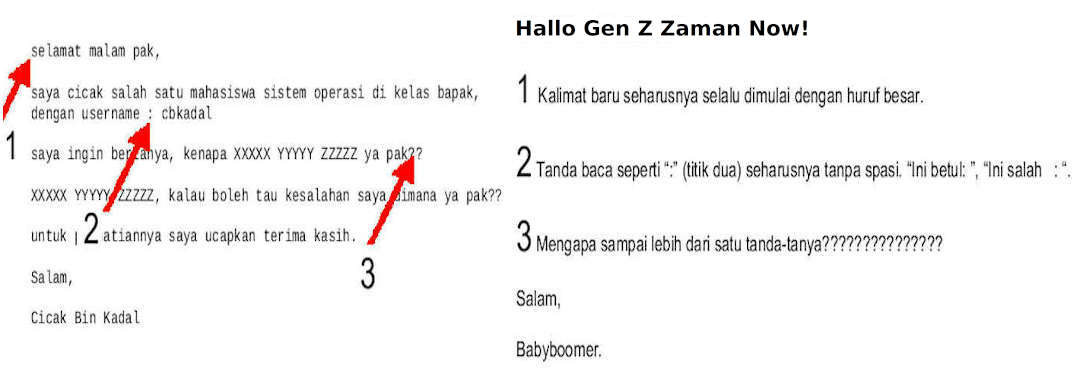
\includegraphics[width=1.01\linewidth]{os-millenial-mail}
\end{figure}
\end{frame}

% XXXXXXXXXXXXXXXXXXXXXXXXXXXXXXXXXXXXXXXXXXXXXXXXXXXXXXXXXXXXXXXXXXXXXXXXXX
\section{Assessment}
\begin{frame}
\frametitle{Assessment}

\begin{itemize}
\item \textbf{11 Weekly Assignments @ 11.11 points}.
\begin{itemize}
\item Assignments will vary from week to week.
\item The assignment deadline will be by the end of every week.
See \url{https://sp.vlsm.org/\#idx02}.
\item Check your points regularly at \url{https://academic.ui.ac.id/}
\item See also, \url{https://sp.vlsm.org/Log/}.
\item \textbf{DO NOT COMPLAIN} weeks after!
\end{itemize}
\item You need to log your weekly activities!
\begin{itemize}
\item See \url{https://doit.vlsm.org/ETC/logCodes.txt}
\item See \url{https://cbkadal.github.io/sp241/TXT/mylog.txt}
\item \textbf{3 SKS} (Units) means 9 hours (540 minutes) per week!
\end{itemize}
\end{itemize}

\end{frame}

% XXXXXXXXXXXXXXXXXXXXXXXXXXXXXXXXXXXXXXXXXXXXXXXXXXXXXXXXXXXXXXXXXXXXXXXXXX
\section{Final Grade}
\begin{frame}
\frametitle{Final Grade (1)}

\begin{itemize}
\item The final grade will be the best 9 out of 11 assignments.
\item Do not ask for any dispensations like a broken computer, circumcision (sunat), cold, competitions 
      (including Gemastik), deadline extension, influenza, lame excuses, marriage, mourning, 
      power failure, remedial, return to the village (mudik), slow network (lemot), two-semester evaluation, umrah,
      weddings, etc. 
\item It also includes: ''It is not my fault but of $\{ X\!: X\ \in\ Lecturer\ \parallel\ Fasilkom\ 
      \parallel\ UI\ \parallel\ Kampus\ Merdeka\ \parallel\ Immigration\ \parallel\ Foreign\ Embassy\ \parallel\ 
      else\, \}$.''
\item \textbf{Two (2) ''spare'' assignments will be more than enough!}
\item In case of emergency, contact your Academic Advisor!
\end{itemize}
\end{frame}

% XXXXXXXXXXXXXXXXXXXXXXXXXXXXXXXXXXXXXXXXXXXXXXXXXXXXXXXXXXXXXXXXXXXXXXXXXX
\begin{frame}
\frametitle{Final Grade (2)}

\begin{itemize}

\item C-2C (C minus to C)
\begin{itemize}
\item Up to 5 points, only if:
\begin{itemize}
\item your grade is between 50.00 and 55.00, and
\item you have a ''good'' track record.
\end{itemize}
\end{itemize}

\item Score Range\\[10pt]
\begin{tabular}{l l l l}
\hline
85 - ... = A & 80 - 85 = A- & 75 - 80 = B+ & 70 - 75 = B \\
65 - 70 = B-      & 60 - 65 = C+ & 55 - 60 = C  & 
50 - 55 = D or C\footnote{C-2C: terms and conditions apply --- void where prohibited by law.}  \\
40 - 50 = D  & 30 - 40 = E  & 20 - 30 = \small E & 00 - 20 = \tiny E   \\
\hline \end{tabular}\\[10pt]

\end{itemize}

\end{frame}

% XXXXXXXXXXXXXXXXXXXXXXXXXXXXXXXXXXXXXXXXXXXXXXXXXXXXXXXXXXXXXXXXXXXXXXXXXX
\begin{frame}[fragile]
\frametitle{The eternal recurring chronic problem}

\textbf{How to avoid receiving emails like the following at the end of the semester after grades have
        been published?}

\begin{figure}
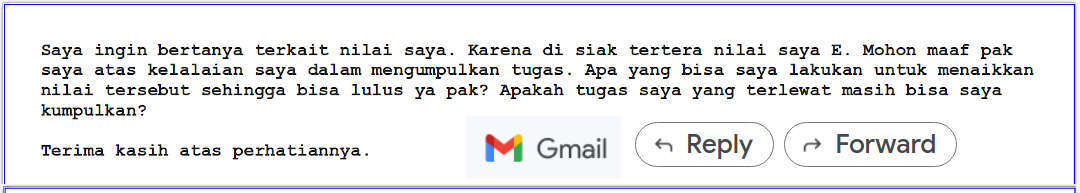
\includegraphics[width=1.01\linewidth]{os-appeal}
\end{figure}

\begin{itemize}
\item Do not ask for any dispensations like a broken computer, circumcision (sunat), cold, competitions
      (including Gemastik), deadline extension, influenza, lame excuses, marriage, mourning,
      power failure, remedial, return to the village (mudik), slow network (lemot), two-semester evaluation, umrah,
      weddings, etc.
\item It also includes: ''It is not my fault but of $\{ X\!: X\ \in\ Lecturer\ \parallel\ Fasilkom\
      \parallel\ UI\ \parallel\ Kampus\ Merdeka\ \parallel\ Immigration\ \parallel\ Foreign\ Embassy\ \parallel\
      else\, \}$.''
\end{itemize}

\end{frame}

% XXXXXXXXXXXXXXXXXXXXXXXXXXXXXXXXXXXXXXXXXXXXXXXXXXXXXXXXXXXXXXXXXXXXXXXXXX
\begin{frame}[fragile]
\frametitle{Grade Examples}

\begin{figure}
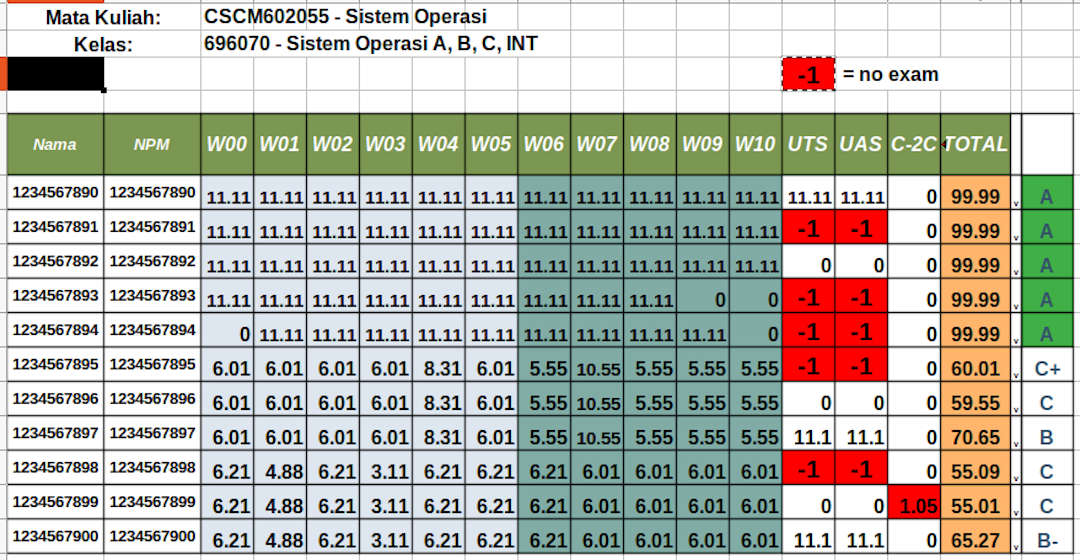
\includegraphics[width=0.94\linewidth]{os-siak}
\end{figure}

\end{frame}

% XXXXXXXXXXXXXXXXXXXXXXXXXXXXXXXXXXXXXXXXXXXXXXXXXXXXXXXXXXXXXXXXXXXXXXXXXX
\section{The Three-Strikes Rule}
\begin{frame}[fragile]
\frametitle{The Three-Strikes Rule}

\begin{figure}
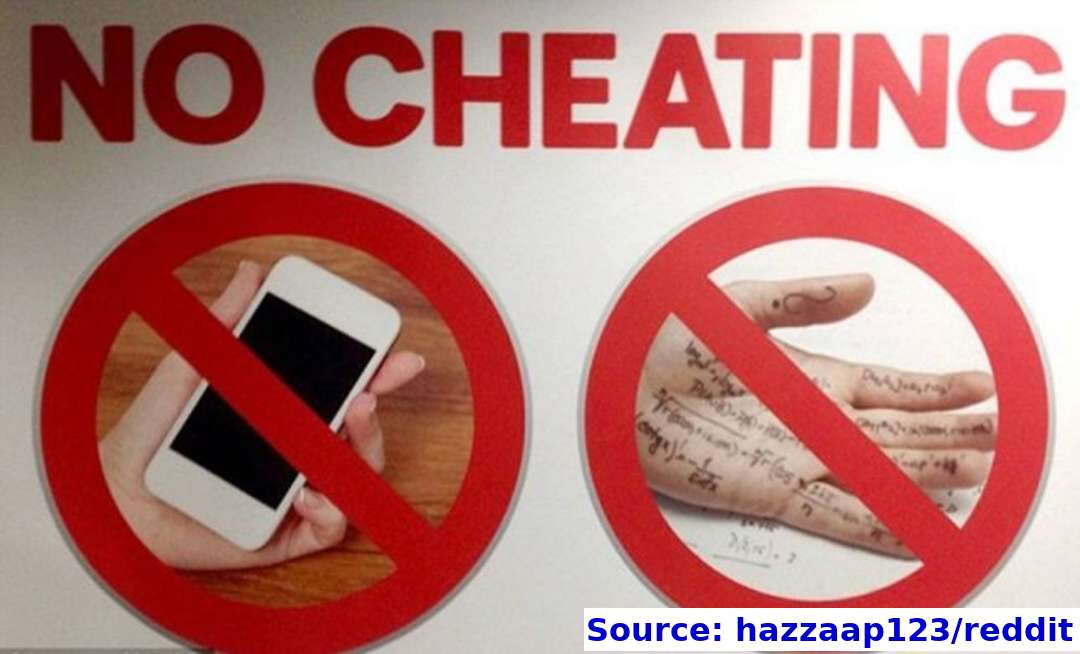
\includegraphics[width=0.30\linewidth]{os-cheating}
\end{figure}

\begin{itemize}
\item All major academic rules violations will be handled directly by the Faculty of Computer Science,
University of Indonesia.
\item ''Accidents'' may happen. There will be warnings for the first two minor violations.
\item Your final grade will be reduced for the third warning.
\item Your final grade will be reduced to "D" for the fourth warning.
\item Five (5) or more warnings will be considered as a significant academic-rules violation.
\end{itemize}

\end{frame}

% XXXXXXXXXXXXXXXXXXXXXXXXXXXXXXXXXXXXXXXXXXXXXXXXXXXXXXXXXXXXXXXXXXXXXXXXXX
\section{Assignments}
\begin{frame}[fragile]
\frametitle{Assignments}
\begin{itemize}
\item There will be no mid-term (UTS) nor final-term (UAS).
      Instead, there will be 11 weekly assignments.
      Your grade will be taken from the best 9 out of 11 assignments.
\item You need to run ''VirtualBox'' on a computer with more than 4GB RAM and up to 64 GB disk space.
\item Each assignment deadline will be by the end of that ''week''.
      The weekly schedule will be at \url{https://sp.vlsm.org/\#idx02}.
\item Submit (push) the assignments to \url{https://github.com/}.
      If you still don't have one, you need to sign up for a \href{https://github.com/}{GitHub} account.
      More information will follow.
\item See the assignment list at \url{https://demOS.vlsm.org/#idx001}.
\end{itemize}
\end{frame}

% XXXXXXXXXXXXXXXXXXXXXXXXXXXXXXXXXXXXXXXXXXXXXXXXXXXXXXXXXXXXXXXXXXXXXXXXXX
\section{This is an elective course!}
\begin{frame}[fragile]
\frametitle{This is an elective course!}

\begin{itemize}
\item You are not required to take this course!
\item This course is not for you if you:
\begin{itemize}
\item do not like the Operating Systems course.
\item do not like to get your hands dirty.
\item do not have enthusiasm nor initiative at all.
\item do not like to ''hack''.
\end{itemize}
\item Cold Feet? Second Guess?  You might want to drop this course now (this week)!
\item This is the way!
\end{itemize}

\end{frame}

% XXXXXXXXXXXXXXXXXXXXXXXXXXXXXXXXXXXXXXXXXXXXXXXXXXXXXXXXXXXXXXXXXXXXXXX
\section{Miscellaneous}
\begin{frame}[fragile]
\frametitle{Out of Topic/Intermezzo/Segue}
\begin{itemize}
\item Semiconductor Scalling:
\begin{itemize}
\item Process Shrink: $10 \mu{}m$ (1971), $250 nm$ (1996), $10 nm$ (2016), $5 nm$ (2020), $3 nm$ (2022).
\item Smaller Devices means:
\begin{itemize}
\item Less space.
\item Less power consumption.
\item More density.
\end{itemize}
\end{itemize}
\item Indonesia:
\begin{itemize}
\item Fairchild Semiconductor Indonesia.
\item National Semiconductor Indonesia.
\item Minister of Manpower (Menteri Tenaga Kerja) 1983–1988.
\end{itemize}
\item Technology:
\begin{itemize}
\item SoC: System on a Chip.
\item SiP: System in a Package.
\item Fab/Foundry: Taiwan Semiconductor Manufacturing Company (TSMC), Ltd.
\begin{itemize}
\item Have No Fab? It is OK! E.g., Marvell Technology, Inc (1995).
\end{itemize}
\item Lithography: ASML Holding, N.V: Advanced Semiconductor Materials Lithography.
\item Optics: Carl Zeiss SMT GmbH (This is NOT Optik Seis, Duh :).
\end{itemize}
\end{itemize}
\end{frame}

% XXXXXXXXXXXXXXXXXXXXXXXXXXXXXXXXXXXXXXXXXXXXXXXXXXXXXXXXXXXXXXXXXXXXXXX
\begin{frame}[fragile]
\frametitle{TSMC Logic Nodes}
\begin{figure}
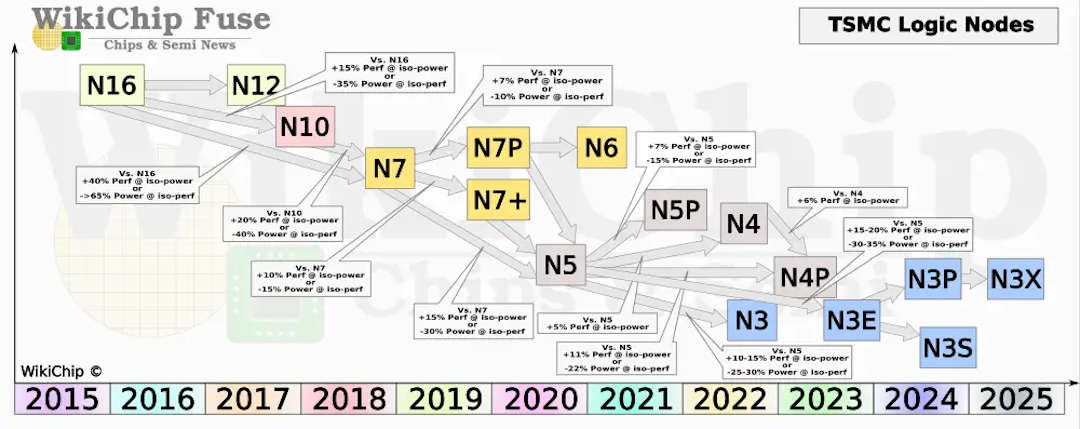
\includegraphics[width=0.95\linewidth]{tsmc_logic_node}
\caption{Source: 
  \href{https://fuse.wikichip.org/wp-content/uploads/2020/04/wikichip_tsmc_logic_node_q1_2020.png}{WikiChip}}
\end{figure}
\end{frame}

% XXXXXXXXXXXXXXXXXXXXXXXXXXXXXXXXXXXXXXXXXXXXXXXXXXXXXXXXXXXXXXXXXXXXXXX
\begin{frame}[fragile]
\frametitle{The Computing Diciplines}
\begin{figure}
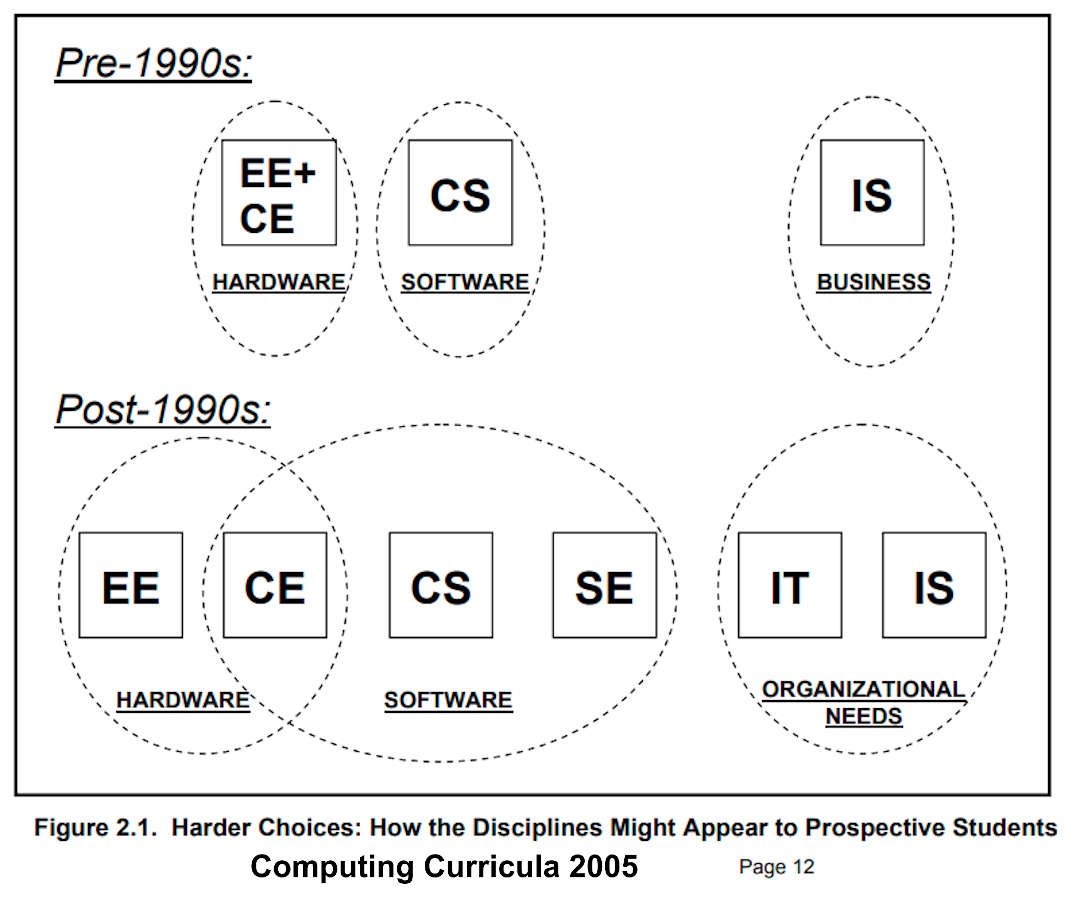
\includegraphics[width=0.59\linewidth]{pic-cc2005}
\caption{The Computing Diciplines}
\end{figure}
\end{frame}

% XXXXXXXXXXXXXXXXXXXXXXXXXXXXXXXXXXXXXXXXXXXXXXXXXXXXXXXXXXXXXXXXXXXXXXXXXX
\end{document}

